\chapter{Methodology}

To gain insights into the proposed methods for researching the appliance of (ND)-Laplace for cluster algorithms we conducted experiments.
The experiment results are used to evaluate our method against other literature.
In this chapter, we explain:
\begin{enumerate}

  \item Datasets
  \item Environmental setup.
  \item For each research question: Description of the different experiments.
  \item For each research question: Results.
\end{enumerate}

\section{Datasets} \label{datasets-section}
For this research, we selected datasets based on the related papers (\ref{theory:literature-review}).
The datasets are sourced from the UCI Machine Learning Repository \citep{noauthor_uci_nodate}.
\begin{enumerate}
  \item Seeds dataset \footnote{http://archive.ics.uci.edu/ml/datasets/seeds}: This dataset was used in several related works and contains 210 samples with 7 (numerical) attributes.
        The dataset contains information about seeds like kernel width and density.
  \item Cardiotocography dataset \footnote{https://archive.ics.uci.edu/ml/datasets/cardiotocography}: This dataset is selected because of the mixed data and amount of instances.
        It has 23 attributes of which 10 are numerical, and has 2126 samples.
        The dataset contains information about measurements of fetal heart rate (FHR) and uterine contraction (UC).
\end{enumerate}
\section{Environmental setup}
For running the experiments we make use of 16GB ram memory and i7-10750H 2.6Ghz processor.
The experiments are run using a Docker container which runs a pre-configured distribution of Linux Alpine.
It includes a pre-installed Anaconda environment for python \footnote{https://github.com/devcontainers/images/tree/main/src/anaconda}\footnote{tag: mcr.microsoft.com/devcontainers/anaconda:0-3}.
We run the container using the dev-container feature for visual-studio code \footnote{https://code.visualstudio.com/docs/devcontainers/containers}.
This allows us to create a reproducible experiment environment.
\subsection{Libraries \& code versions}
We use python version 3.9.13 with Jupyter notebook for creating a reproducible experimental environment.
The packages for python are:
\begin{enumerate}
  \item Scikit-learn: 1.0.*
  \item Yellow-brick: 1.5
  \item Numpy: 1.24.*
  \item Pandas: 1.4.*
  \item Seaborn: 0.11.*
  \item Mathplotlib: 3.5.*
\end{enumerate}

\section{Methods}
This section explains what methods/ algorithms we used and how we evaluate them.
\subsection{Clustering methods}
\todo[inline]{In progress}
For the three different algorithms: K-Means, \gls{ap} and \gls{dbscan} we analyzed the most important decisions regarding parameter selection.
In this section, we give a short list and explanation of the different parameters we used throughout the experiments.
For all three Scikit-learn was used, and for each of them we also provide the underlying formula.
\subsubsection{K-Means}
\begin{equation}
  \sum_{i=0}^{n}\min_{\mu_j \in C}(||x_i - \mu_j||^2)
\end{equation}
\begin{table}[h]
  \begin{tabular}{|l|p{6cm}|l|l|}
    \hline
    Parameter & Description                          & Value                                                 & Dataset   \\ \hline
    K-value   & Calculated based on an "elbow" plot. & 4 (see figure \ref{hyperparameters:k-means-dataset1}) & Dataset 1 \\ \hline
    K-value   & TODO                                 & ??                                                    & Dataset 2 \\ \hline
    K-value   & TODO                                 & ??                                                    & Dataset 3 \\


    \hline
  \end{tabular}
  \caption{K-Means hyperparameters for dataset 1 - 3}
  \label{tab:kmeans-formula-dataset-2}
\end{table}

\subsubsection{Affinity Propagation}
As specified in section \ref{theory:clustering-ap}, the clustering algorithm has two types of similarity.
The responsibility is calculated by the following formula:
\begin{equation}
  r(i, k) \leftarrow s(i, k) - max [ a(i, k') + s(i, k') \forall k' \neq k ]
\end{equation}
Then the availability is given using this formula:
\begin{equation}
  a(i, k) \leftarrow min [0, r(k, k) + \sum_{i'~s.t.~i' \notin \{i, k\}}{r(i', k)}]
\end{equation}
And iteratively calculated while considering the damping factor.
\begin{table}[h]
  \begin{tabular}{|l|p{6cm}|l|l|}
    \hline
    Parameter      & Description                                                                                & Value & Dataset   \\
    \hline
    Preference     & We decided to use the median similarity as described in section \ref{theory:clustering-ap} & TODO  & dataset 1 \\
    \hline
    Preference     & ""                                                                                         & TODO  & dataset 2 \\
    \hline
    Preference     & ""                                                                                         & TODO  & dataset 3 \\
    \hline
    Damping factor & Default value as specified in section \ref{theory:clustering-ap}                           & 0.5   & dataset 1 \\
    \hline
    Damping factor & ""                                                                                         & 0.5   & dataset 2 \\
    \hline
    Damping factor & ""                                                                                         & 0.5   & dataset 3 \\
    \hline
  \end{tabular}
  \caption{Affinity Propagation hyperparameters for datasets 1 - 3}
  \label{tab:ap-formula-sklearn}
\end{table}
\subsubsection{DBSCAN}
\todo[inline]{Give algorithm formula}
\todo[inline]{Describe how/why we choose for OPTICS}
\begin{table}[h]
  \begin{tabular}{|l|p{6cm}|l|l|}
    \hline
    Parameter      & Description                                                                                                    & Value                                                  & Dataset   \\
    \hline
    Epsilon        & Decided using the k-distance plot                                                                              & 0.9 (see figure \ref{hyperparameters:DBSCAN-dataset1}) & Dataset 1 \\
    \hline
    Epsilon        & ""                                                                                                             & TODO                                                   & Dataset 2 \\
    \hline
    Epsilon        & ""                                                                                                             & TODO                                                   & Dataset 3 \\
    \hline
    Minimum points & Decided using the formula $minPts = n * 2$, where n is the number of features (\ref{theory:clustering-dbscan}) & 4                                                      & Dataset 1 \\
    \hline
    Minimum points & ""                                                                                                             & 6                                                      & Dataset 2 \\
    \hline
    Minimum points & ""                                                                                                             & 10                                                     & Dataset 3 \\
    \hline
  \end{tabular}
  \caption{DBSCAN  hyperparameters for datasets 1 - 3}
  \label{tab:dbscan-formula-sklearn}
\end{table}

\newpage
\subsection{Evaluation}
With differential privacy, it is a trade-off of utility versus privacy.
Therefore, for the evaluation of the 2D/3D-Laplace algorithms, we compare both criteria to achieve a consensus between utility and privacy.
To reduce the measurement bias of results we executed them 10 times for multiple privacy budgets and report the average for each \citep{9679364}.

\begin{enumerate}
  \item All experiments are performed 10 times and the average is reported.
  \item All experiments are performed per privacy budget (epsilon).
        We have a fixed list for this: ${0.05, 0.1, 0.5, 1, 2, 3, 5, 7, 9}$.
\end{enumerate}

\subsubsection{Utility}
Based on section \ref{theory:evaluate}, we can conclude that the corresponding literature mainly evaluates one clustering algorithm and not multiple ones.
Furthermore, it can be concluded that if we only want to measure the coherence of the clusters, we can use an internal validation method. If we want a concrete measurement compared to the non-private version, an external validation method can be used.
Both measurements are important to evaluate, so we use both external and internal validation. \newline

\textbf{External validation:}
We will use both \gls{ari} and \gls{ami} different strengths we evaluate both.
For the validation we want to validate how much utility we lose using our method for a given privacy budget ($\epsilon$).
Therefore, we evaluate smaller sets of data to measure this for local perturbation.
To compensate for this, the adjusted version is used for both Rand Index and Mutual Information.
%The clustering algorithm is trained using the plain data and functions as the ground truth \citep{9646464,sun_distributed_2019}.
%Because of this, we are being able to calculate the \gls{ami} and compare the centroids between the non-private and privately trained clusters.
The implementation for these metrics is provided by the Scikit-learn package.
With the underlying formulas:
\begin{equation}
  AMI(U, V) = \frac{MI(U, V) - E(MI(U, V))}{avg(H(U), H(V)) - E(MI(U, V))}
\end{equation}
\capequation{Adjusted Mutual Information formula \citep{vinh_information_nodate-2,hubert_comparing_1985-1}}
\begin{gather}
  RI = \frac{a + b}{C^{n}_{2}} \\
  ARI = \frac{RI - E(RI)}{max(RI) - E(RI)}
\end{gather}
\capequation{(Adjusted) Rand Index formula \citep{rand_objective_1971, hubert_comparing_1985-1}}

\textbf{Internal validation:}
To evaluate the cluster algorithms, we use \gls{chi} and silhouette score.
The expectation is that both will give a similar result, but they measure the cluster coherence in different ways. \newline
%%The second way to measure utility is to calculate the error between the non-private and perturbed data \citep{9679364,sun_distributed_2019,xia_distributed_2020-1}.
%There are several methods to do this (See \ref{theory:evaluate}), but we use the \gls{aee}.
%As with \gls{ami} we run the calculations for multiple privacy budgets 10 times and report the average for each budget.
%\todo[inline]{Explain why AEE and not RE}
\textbf{Comparison:}
It is important to compare our mechanism to comparable methods.
Therefore, we compare our results with similar methods that are proposed in the literature, based on these criteria:
\begin{enumerate}
  \item It should work with n-dimensional data.
  \item It should have an open-source implementation to be able for us to compare it.
  \item The method should be general-purpose (e.g. not only mean-estimation) and work preferably locally.
\end{enumerate}
For checking these requirements, we have defined the tables (\ref{tab:summary_table_dp}, \ref{tab:summary_table_kmeans}) as a summary of our literature review.
Based on this, it can be concluded that the "piecewise" mechanism is the only one that meets this requirement.

\subsubsection{Privacy}
Privacy is hard to quantify, but we can measure the privacy loss/gain by calculating the Euclidean distance between the non-perturbed data and the perturbed data.
In addition, we evaluate privacy by simulating a membership inference attack and calculating the adversary advantage. \newline
\textbf{Privacy distance:} We calculate the Euclidean average difference between non-perturbed data and perturbed data.
This is measured for each epsilon. \newline
\textbf{Membership inference attack (adversary advantage):}
%\begin{algorithm}[H]
  \caption{Black-box inference attack}\label{alg:shokri-mi}
  \begin{algorithmic}
    \Ensure $z$
    \State $x_{target}, y_{target}, x_{shadow}, y_{shadow} = split(X)$ \Comment 75\% shadow data
    \State $x_{target-train}, y_{target-train} = split(xy_{target})$ \Comment 12.5\% train data
    \State $x_{target-test}, y_target_test = split(xy_{target})$ \Comment 12.5\% test data
    \State $Z = 2/3nD-Laplace(x_{target-train})$ 
    \State $private_classifier = RandomForestClassifier(Z, y_{target-train})$ \Comment See scikit-learn (\textbf{Bron})
    \For{three times}
      \State $dataset_{shadow} = generate_shadow_datasets$ \Comment using ART implementation
    \EndFor

  \end{algorithmic}
\end{algorithm}
We used the MIA that was proposed by Shokri et al. with the implementation that was provided by Adversarial Robustness Toolkit (ART) \citep{nicolae_adversarial_2019}.
An earlier study also explored this attack with as goal to evaluate differential privacy.
Similar to this attack, we train a classifier with perturbed data and evaluate it using non-perturbed data (test-data / shadow-data) \citep{zhao_not_2020}.
We consider a semi-surpervised setup (figure \ref{figure:MIA-semi-supervised}), where we train a classifier with the perturbed data and evaluate it using non-perturbed data (test-data / shadow-data).
For the classifier, we use a RandomForestClassifier, because this classifier is not yet applied for shadow model attacks \citep{rigaki_survey_2021}.
Finally, we evaluate the adversary advantage (percentage) using $TPR - FPR$ \citep{yeom_privacy_2018}.
\begin{enumerate}
  \item TPR: The amount the attacker inferred the member data correctly (the private training data).
  \item FPR: The amount the attacker inferred the non-member data correctly (the non-private test data).
\end{enumerate}
\todo[inline]{Include ROC plot rationale}
A visual setup of the experiment is given in figure: \ref{figure:mi-attack}

\begin{figure}
  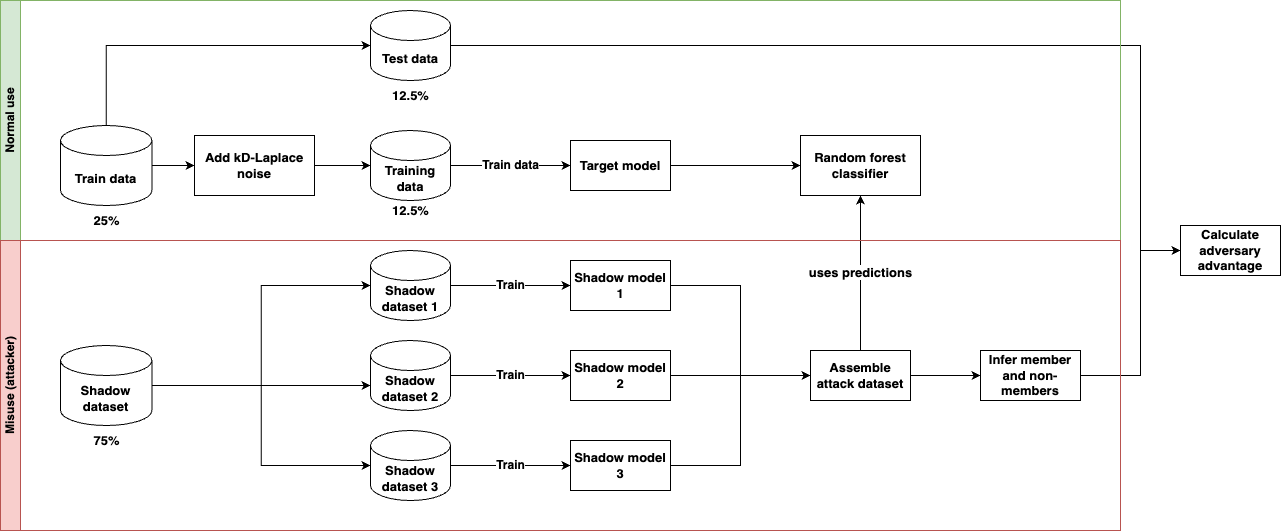
\includegraphics[width=1.2\textwidth]{Method/images/MI-setup.png}
  \caption{Member inference attack using shadow models. The green swim lane illustrates the normal setup and the red swim lane projects the adversary steps.}
  \label{figure:mi-attack}
\end{figure}
\newpage
%Therefore, we analyze our method according to a popular attack: Membership inference attack.
%For this purpose, we make use of a black-box Member inference attack, called "HopSkipJump" \citep{chen_hopskipjumpattack_2020,li_membership_2021}.
%This attack is evaluated using a semi-supervised setup, as proposed in this figure: \ref{fig:unsupervised-mia-attack}.
%We will make use of a decision tree model for classification but can be replaced by any other classification model.
%Both the private and non-private trained models are evaluated based on the true positive rate (TPR) and false positive rate (FPR).
%Respectively meaning, the TPR is higher if the MIA is successful and likewise the FPR if the MIA is unsuccessful.
%We hypothesize that the private model leverages a higher FPR in comparison to the non-private variant.
%Therefore, it is more convenient to apply the geo-indistinguishability as an error metric provided in \ref{eq:geo-as-an-error}.
\subsection{Scaling}
Because we use a distance metric, we need to apply some data standardization.
For this purpose, we use standard scaling provided by the Scikit-learn package \footnote{https://scikit-learn.org/stable/modules/preprocessing.html}.
This is only for clustering, so it is applied after all the perturbation algorithms.
\subsection{Research question 1}
For research question 1 we evaluate the following methods:
\begin{enumerate}
  \item 2D-Laplace: algorithm \ref{alg:2d-laplace}.
  \item 2D-Laplace: truncated algorithm \ref{alg:find-outside-domain-laplace} and \ref{alg:grid-remapping-laplace}.
  \item Piecewise: algorithm \todo{Provide piecewise}.
\end{enumerate}
\mycomment{
  We propose several solutions for open issues based on the theoretical framework. \newline
  \subsubsection{Choosing r: } Based, on the idea of chatzikokolakis et al. to lower the size of the radius if the place is crowded, we can do the same with clustering.
  For this, we could use a metric like the standard division.
  This metric does exactly this, by providing the deviation from the mean:

  This metric increases based on clutteredness of the data, which allows us to generate a radius $r$ automatically regardless of domain.
  Therefore, we depend on the configurability of epsilon entirely on privacy level $l$.
  The generic standard deviation can be defined as:
  \begin{equation}
    \sigma = \sqrt{\frac{\sum{(x_i - \mu)^2}}{n}}
  \end{equation}
  The $\sigma$ being our diameter $d$, the radius $r$ is then calculated as $\frac{d}{2}$. \newline
}
\mycomment{\subsubsection{Truncation:}
  We explained the theory for truncation earlier in paragraph \ref{theory:truncation}.
  The methods proposed work correctly for a geographic map where other (historic) locations for remapping are available.

  However, it is difficult to apply this to data clustering.
  The number of data points is not known beforehand, so we may remap to a location that is too far away.
  This way we lose important distance information, which hurts the clustering.
  Also, the truncation threshold is so clear (the points are outside the known 2D domain), that we do not have to rely on historical data for remapping.
  Our algorithm can be much simpler by re-calculating the noise until it will be within the domain:
}
\mycomment{
  \begin{equation}
    T(x_{max}, x_{min}, z, x_0) \begin{cases} z &\text{if } 0 < 1 \\ T(x_{max}, x_{min}, planarLaplace(epsilon, x_0), x_0)  &\text{else} \end{cases}
  \end{equation}
}
%\begin{algorithm}
  \caption{Truncation algorithm ($T(\min, \max, x_0, z)$) for clustering with planar Laplace}\label{alg:truncaction-rq1}
  \begin{algorithmic}
    \Ensure $z$
    \State $x_1, y_1 \gets x_{min}$
    \State $x_2, y_2 \gets x_{max}$
    \State $z_x, z_y \gets z$
    \If{$x_1 < z_x < x_2$ and $y_1 < z_y < y_2$}
    \State \Return $z$
    \Else
    \State $x, y \gets x_0$
    \State $z_2 \gets LP(\epsilon, x, y)$ \Comment See formula 3.3.
    \State \Return $T(x_{min}, x_{max}, x_0, z_2)$ \Comment Rerun recursively
    \EndIf
  \end{algorithmic}
\end{algorithm}
%This algorithm uses $x_{min}$ and $x_{max}$ to re-calculate the points within the domain using respectively the minimum X/Y and maximum X/Y.
%An example of this is visualized:
%\begin{figure}[h]
%  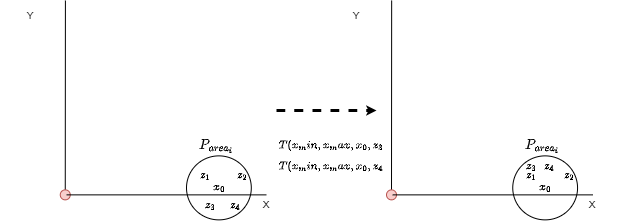
\includegraphics[width=0.8\textwidth]{Method/images/truncation-rq1.png}
%  \label{fig:truncation}
%  \centering
%  \caption{Representation of the remapping algorithm for clustering for points $z_3$ and $z_4$ }
%\end{figure}

%\subsubsection{Probability metric $K(x)(Z)$}
%\todo[inline]{Explain the probability metric $K$ we used}

%\newpage
%\subsubsection{Algorithm}
%The full algorithm for the perturbation:
%\begin{algorithm}[H]
  \caption{Full algorithm for perturbing cluster data based on planar/2D-Laplace \citep{DBLP:journals/corr/abs-1212-1984}}\label{alg:rq1}
  \begin{algorithmic}
    \Require $x \in X$  \Comment 2D array of points
    \Require $l \in R^ +$
    \Ensure $z \in Z$ \Comment 2D array of perturbed points
    \State $r = \frac{\sigma}{2}$ \Comment formula 4.1
    \State $\epsilon = \frac{l}{r}$ \Comment Calculating privacy budget \citep{DBLP:journals/corr/abs-1212-1984}
    \State $x_{min} \gets min(X)$
    \State $x_{max} \gets max(X)$
    \State $Z \gets []$
    \For{$point_i \in X$}
    \State $\theta \gets [0, \pi2]$       \Comment Random noise for $\theta$
    \State $p \gets [0, 1]$
    \State $z_i \gets C{_\epsilon}{^{-1}}(p)$       \Comment formula 3.2
    \State $z_i \gets T(x_{min}, x_{max}, point_i, z_i)$ \Comment algorithm 1.
    \State $x_{perturbed} \gets point_{i_x} + (z_{i_x} * \cos(\theta)) $ \Comment add noise to x-coordinate
    \State $y_{perturbed} \gets point_{i_y} + (z_{i_y} * \sin(\theta)) $ \Comment add noise to y-coordinate
    \State append $x_{perturbed}, y_{perturbed}$ to Z
    \EndFor
    \State \Return Z
  \end{algorithmic}
\end{algorithm}
%% We apply the theory for planar laplace proposed by \citep{DBLP:journals/corr/abs-1212-1984}

\subsection{Research question 2}
The setup for research question 2 is similar to research question 1, but we use 3D-Laplace instead of 2D-Laplace.
\begin{enumerate}
  \item 3D-Laplace: algorithm \ref{alg:3d-laplace}.
  \item 3D-Laplace: truncated algorithm \ref{alg:find-outside-domain-laplace} and \ref{alg:grid-remapping-laplace}.
  \item Piecewise: algorithm.
\end{enumerate}
\newpage
\subsection{Research question 3}
%\todo[inline]{Added ideas for research question 3}
In this research question, we compare the behavior of our mechanism with what we have observed in the literature for similar mechanisms.
To do this, we have formulated several hypotheses.
\begin{enumerate}
  \item The privacy leakage (adversary advantage) increases for a higher number of dimensions:
        It is expected that privacy leakage increases with the number of dimensions, based on our own observation (\ref{theory:privacy-utility-nd}).
        \todo[inline]{Also include literature}
        \mycomment{\item The boundary distance attack proposed by Choquette et al. yields better results on our data.
        We evaluated research questions 1 and 2 using the attack model proposed by Shokri et al. \cite{shokri_membership_2017}.
        However, Choquette et al. proposed a new attack model that is more suitable for our data \cite{choquette_privacy-preserving_2019}.
        We expect that the results of this attack model are better than the results of the attack model proposed by Shokri et al.}
  \item Adding optimal remapping improves utility without sacrificing privacy \todo{link}.
        \todo[inline]{Include more information}
\end{enumerate}
In addition to testing the hypotheses, we also want to investigate the behavior of our mechanism in more detail.
\begin{enumerate}
  \item Research the applicability of the mechanism for other cluster algorithms, like hierarchical clustering.
  \item Research the impact of the data shape on privacy leakage.
  \item Explore options to extend the method to support categorical data.
  \item Explore options to extend the method to support binary data.
        %\item Research possibility to include the privacy mass: \ref{equation:privacy-mass-a}.
\end{enumerate}
